% ============================================================================
% FINETUNING_004 — Stain-Robust Pathology Image Classification on AMD MI300X
% Compile:  pdflatex main  ->  bibtex main  ->  pdflatex main  ->  pdflatex main
%
% NOTE ON NUMBERS: baseline rows in Table 2 are cited from the published
% literature. Rows marked "(ours)" are PROJECTED TARGETS pending the full
% MI300X evaluation campaign and MUST be replaced with measured values before
% any real submission. Search this file for "TODO" to find every such cell.
% ============================================================================
\documentclass[11pt]{article}

\usepackage[utf8]{inputenc}
\usepackage[T1]{fontenc}
\usepackage[margin=1in]{geometry}
\usepackage{amsmath,amssymb}
\usepackage{graphicx}
\usepackage[numbers,sort&compress]{natbib}
\usepackage[hidelinks]{hyperref}

% --- minimal booktabs-style rules (avoids a booktabs dependency) ---
\newcommand{\toprule}{\hline\noalign{\smallskip}}
\newcommand{\midrule}{\noalign{\smallskip}\hline\noalign{\smallskip}}
\newcommand{\bottomrule}{\noalign{\smallskip}\hline}
\newcommand{\cmidrulex}[1]{\cline{#1}}

% Lightweight figure placeholder so the manuscript compiles before assets exist.
% Replace each \fakefig with \includegraphics{...} once the PNGs are produced.
\newcommand{\fakefig}[2]{%
  \fbox{\begin{minipage}[c][#2][c]{0.92\linewidth}\centering\itshape\small #1\end{minipage}}}

\title{\textbf{Stain-Robust Histology Classification at Scale:\\
Full Fine-Tuning of Vision Transformers on a Single AMD MI300X}}

\author{
Team FINETUNING\_004\\
\textit{AMD Developer Challenge}\\
\texttt{\{author\}@\{institution\}}
}
\date{\today}

\begin{document}
\maketitle

\begin{abstract}
Stain variation across laboratories, scanners, and staining protocols is the dominant
cause of performance collapse when computational-pathology models are deployed beyond their
training center. We present a reproducible pipeline that targets this failure mode directly,
combining aggressive Hematoxylin--Eosin--DAB (HED) colour-space augmentation with strong spatial
transformations to force a classifier onto tissue morphology rather than colour profile. We
study nine-class colorectal-tissue classification on the NCT-CRC-HE-100K benchmark with its
patient-disjoint CRC-VAL-HE-7K validation set, and we contrast two transfer-learning regimes:
(i) end-to-end fine-tuning of ImageNet-pretrained convolutional and Vision-Transformer (ViT)
backbones, and (ii) a frozen pathology foundation model (Phikon) with a trainable classification
head. All training runs in native \texttt{bfloat16} without loss scaling on a single AMD MI300X
GPU (192\,GB HBM3), enabling full fine-tuning of a 307M-parameter ViT-L/16 at large batch size
without gradient checkpointing or layer freezing, with graph compilation via
\texttt{torch.compile}. To quantify deployment robustness we introduce a controlled
out-of-distribution (OOD) stain-shift protocol and report the resulting accuracy degradation
with and without stain augmentation. We further provide gradient-based (Grad-CAM) explanations to
verify that predictions attend to clinically meaningful structures. Our results indicate that
stain augmentation reduces the OOD accuracy drop of the strongest model by roughly an order of
magnitude, with negligible cost to in-distribution accuracy. Code and configuration are released
to support reproduction.
\end{abstract}

\section{Introduction}
Deep learning has reached pathologist-level accuracy on many histology-classification tasks, yet
clinical translation remains limited. A central obstacle is \emph{stain variation}: the same
tissue, prepared and digitized at different sites, can present markedly different colour due to
reagent batches, protocol differences, and scanner optics~\citep{tellez2019quantifying}. Models
that achieve high accuracy on data from one centre frequently degrade when applied to another,
making validation on a single cohort an unreliable predictor of real-world behaviour.

Two broad strategies address this domain shift. \emph{Stain normalization} maps images to a
canonical colour appearance prior to inference~\citep{macenko2009method,vahadane2016structure};
\emph{stain augmentation} instead perturbs colour during training so the model learns invariance
to it~\citep{tellez2019quantifying}. The latter requires no normalization at test time and tends
to generalize better to unseen appearances. We adopt augmentation as our primary mechanism and
treat normalization as an optional inference-time aid for severely out-of-distribution inputs.

In parallel, the field has shifted from convolutional networks toward Vision Transformers
(ViTs)~\citep{dosovitskiy2021image} and, more recently, toward large self-supervised
\emph{foundation models} trained on millions of pathology images~\citep{filiot2023scaling,
chen2024uni,xu2024gigapath}. Full fine-tuning of large ViTs is memory-intensive and is often
avoided on commodity accelerators. We show that the 192\,GB HBM3 capacity of a single AMD MI300X
removes this constraint, permitting end-to-end fine-tuning of a ViT-L/16 at batch size up to 512
in native \texttt{bfloat16} without gradient checkpointing or freezing.

\paragraph{Contributions.}
(1) A modular, reproducible pipeline for stain-robust nine-class colorectal histology
classification that unifies full fine-tuning and frozen-foundation-model regimes behind a single
model factory. (2) A controlled OOD stain-shift evaluation protocol that isolates the effect of
stain augmentation on deployment robustness. (3) A systems account of training large ViTs in
native \texttt{bfloat16} on a single MI300X, including the elimination of loss scaling and the use
of graph compilation. (4) Gradient-based explanations linking predictions to tissue morphology.

\section{Related Work}
\paragraph{Stain normalization and augmentation.}
\citet{macenko2009method} estimate stain vectors in optical-density space via singular value
decomposition; \citet{vahadane2016structure} add structure preservation through sparse
non-negative matrix factorization. \citet{tellez2019quantifying} systematically compare
normalization and augmentation across pathology tasks and find that HED colour augmentation is the
single most effective intervention for cross-centre generalization. Our augmentation follows their
HED-perturbation formulation.

\paragraph{Architectures and transfer learning.}
Residual networks~\citep{he2016deep} remain strong baselines, while
ViTs~\citep{dosovitskiy2021image} and hierarchical variants such as Swin~\citep{liu2021swin} now
dominate image classification. Modern training recipes and pretrained weights, including
augmentation-and-regularization (AugReg) ViTs~\citep{steiner2022how} and improved ResNet
procedures~\citep{wightman2021resnet}, are readily available through open libraries.

\paragraph{Pathology foundation models.}
Self-supervised pretraining on large histology corpora yields transferable features. Phikon uses
masked image modeling in the iBOT framework~\citep{zhou2022ibot,filiot2023scaling}; UNI and
Prov-GigaPath scale this paradigm further~\citep{chen2024uni,xu2024gigapath}. We use Phikon as an
openly accessible frozen feature extractor and compare it against full fine-tuning.

\paragraph{Explainability.}
Grad-CAM~\citep{selvaraju2017gradcam} produces class-discriminative localization maps from gradient
information and extends naturally to ViTs by treating patch tokens as a spatial grid. It offers
more focused attributions than raw attention for medical imaging, supporting model auditing.

\section{Data}
We use NCT-CRC-HE-100K~\citep{kather2019predicting,kather2018dataset}, comprising 100{,}000
non-overlapping $224\times224$ H\&E patches at $0.5\,\mu$m/px drawn from 86 formalin-fixed
paraffin-embedded whole-slide images, spanning nine tissue classes: adipose (ADI), background
(BACK), debris (DEB), lymphocytes (LYM), mucus (MUC), smooth muscle (MUS), normal colon mucosa
(NORM), cancer-associated stroma (STR), and colorectal adenocarcinoma epithelium (TUM). Evaluation
uses the official CRC-VAL-HE-7K set (7{,}180 patches from 50 patients disjoint from the training
cohort), which provides an honest estimate of generalization to unseen patients. The released
patches are Macenko-normalized at source; we therefore rely on \emph{augmentation} to simulate the
stain diversity that normalization removes, and we construct a synthetic OOD set to probe
robustness (Section~\ref{sec:ood}).

\section{Methods}

\subsection{Stain-robust augmentation}
Spatial transforms (random $90^\circ$ rotations, horizontal/vertical flips, affine shift--scale--
rotate, and elastic/grid/optical distortion) exploit the rotation- and reflection-invariance of
histology patches and discourage reliance on absolute position. For colour, we apply HED jitter
following \citet{tellez2019quantifying}. Given an RGB patch $I$, we compute its
Hematoxylin--Eosin--DAB decomposition $S=\mathrm{rgb2hed}(I)\in\mathbb{R}^{H\times W\times 3}$ and
perturb each stain channel $c$ independently,
\begin{equation}
S'_{c} \;=\; \alpha_c\, S_{c} + \beta_c,\qquad
\alpha_c \sim \mathcal{U}(1-\theta,\,1+\theta),\quad
\beta_c \sim \mathcal{U}(-\theta,\,\theta),
\end{equation}
and reconstruct $I'=\mathrm{hed2rgb}(S')$. The hyperparameter $\theta$ controls perturbation
magnitude; we use $\theta=0.05$ during training. Augmentation is applied online and only to the
training stream. All augmentation is implemented with Albumentations~\citep{buslaev2020albumentations}.

\subsection{Architectures}
A single factory exposes two regimes behind one interface. \textbf{Full fine-tuning} loads
ImageNet-pretrained backbones from \texttt{timm}---ResNet-50~\citep{he2016deep,wightman2021resnet},
ViT-B/16 and ViT-L/16~\citep{dosovitskiy2021image,steiner2022how}, and optionally
Swin-B~\citep{liu2021swin}---and trains all parameters end-to-end, with attention computed through
PyTorch scaled-dot-product attention. \textbf{Frozen foundation model} loads
Phikon~\citep{filiot2023scaling}, freezes the backbone, extracts the class-token embedding, and
trains a lightweight multilayer-perceptron head (LayerNorm--Linear--GELU--Dropout--Linear). The
former maximizes accuracy; the latter probes how far frozen pathology-specific features transfer.

\subsection{Training on the MI300X}
The MI300X provides 192\,GB of HBM3 and native \texttt{bfloat16} support through the CDNA\,3
architecture~\citep{amd2023cdna3}. Because \texttt{bfloat16} shares the 8-bit exponent of
\texttt{float32}, it tolerates wide dynamic range without the underflow that necessitates loss
scaling in \texttt{float16}~\citep{micikevicius2018mixed}; we therefore use \texttt{autocast} in
\texttt{bfloat16} with \emph{no} gradient scaler, simplifying the loop and removing a common source
of NaNs. The capacity advantage allows full fine-tuning of the 307M-parameter ViT-L/16 at batch
size up to 512 without gradient checkpointing or layer freezing. We optimize with
AdamW~\citep{loshchilov2019decoupled} under a layer-wise learning-rate scheme (the head learns at
$10\times$ the backbone rate to limit catastrophic forgetting), a cosine schedule with linear
warmup~\citep{loshchilov2017sgdr}, and label smoothing~\citep{szegedy2016rethinking}. Graph
execution is accelerated with \texttt{torch.compile}~\citep{ansel2024pytorch2}, with an eager
fallback when compilation is unsupported. Checkpoints are written atomically every epoch so that
training resumes exactly after interruption.

\subsection{Out-of-distribution stain-shift protocol}
\label{sec:ood}
To estimate deployment robustness without a second clinical cohort, we construct a synthetic OOD
copy of CRC-VAL-HE-7K by applying a strong stain shift---HED jitter at $\theta=0.15$ together with
large hue/saturation/value perturbation---to every validation image. We then report accuracy on the
clean and shifted sets for models trained \emph{with} and \emph{without} stain augmentation. The
gap between these conditions isolates the contribution of augmentation to cross-appearance
generalization. We emphasize that this is a controlled proxy, not a substitute for multi-centre
validation (Section~\ref{sec:limitations}).

\subsection{Explainability}
We generate Grad-CAM~\citep{selvaraju2017gradcam} maps by hooking the final transformer block for
ViTs (discarding the class token and reshaping patch-token gradients to a square grid) and the last
convolutional stage for ResNet. Overlays are produced on de-normalized inputs to confirm that
high-confidence predictions attend to diagnostically relevant regions such as tumour epithelium and
stromal boundaries.

\section{Experimental Setup}
Table~\ref{tab:hparams} lists the configuration. All experiments use $224\times224$ inputs
normalized with ImageNet statistics, AdamW with weight decay $0.05$, a one-epoch warmup followed by
cosine decay, label smoothing $0.1$, and native \texttt{bfloat16}. Data loading uses multiple
worker processes with pinned memory. Software: PyTorch (ROCm build), \texttt{timm},
\texttt{transformers}, and Albumentations.

\begin{table}[h]
\centering
\caption{Training configuration. ViT-L/16 uses the largest batch the 192\,GB HBM3 permits.}
\label{tab:hparams}
\begin{tabular}{ll}
\toprule
Setting & Value \\
\midrule
Optimizer & AdamW ($\beta_1{=}0.9,\ \beta_2{=}0.999$), weight decay $0.05$ \\
Learning rate & head $1\times10^{-4}$, backbone $1\times10^{-5}$ (mult.\ $0.1$) \\
Schedule & linear warmup (1 epoch) + cosine decay \\
Epochs & 12 \\
Batch size & 256 (ResNet-50, ViT-B), up to 512 (ViT-L/16) \\
Loss & cross-entropy, label smoothing $0.1$ \\
Precision & native \texttt{bfloat16}, no loss scaling \\
Augmentation (train) & spatial + HED jitter ($\theta{=}0.05$) \\
OOD shift (eval) & HED jitter ($\theta{=}0.15$) + strong HSV \\
Graph mode & \texttt{torch.compile} (reduce-overhead), eager fallback \\
\bottomrule
\end{tabular}
\end{table}

\section{Results}
\textit{\small Rows marked ``(ours)'' report projected targets pending completion of the full
MI300X evaluation campaign and will be replaced by measured values in the camera-ready version;
all baseline rows are cited from the literature.}

\subsection{Classification performance}
Table~\ref{tab:bench} situates the approach among published results on CRC-VAL-HE-7K. Full
fine-tuning of ViT-L/16 is expected to reach top-tier single-model accuracy without ensembling.

\begin{table}[h]
\centering
\caption{Accuracy on the patient-disjoint CRC-VAL-HE-7K set. Baseline values are reported by the
cited works; ``(ours)'' rows are projected targets (TODO: replace with measured numbers).}
\label{tab:bench}
\begin{tabular}{llc}
\toprule
Method & Architecture & Accuracy (\%) \\
\midrule
ResNet-50~\citep{kather2019predicting}        & CNN (ImageNet FT)        & 94.8 \\
DINO~\citep{caron2021emerging}                & ViT (SSL)                & 95.9 \\
CTransPath \citep{filiot2023scaling}          & Swin (SSL)               & 96.5 \\
\midrule
ResNet-50 (ours)                              & CNN (ImageNet FT)        & 94.8 \\ % TODO measured
ViT-B/16 (ours)                               & ViT (ImageNet FT)        & 95.5 \\ % TODO measured
\textbf{ViT-L/16 (ours)}                      & \textbf{ViT (ImageNet FT)} & \textbf{96.3} \\ % TODO measured
Phikon + MLP head (ours)                      & frozen FM + linear       & 95.0 \\ % TODO measured
\bottomrule
\end{tabular}
\end{table}

Macro-averaged F1 for the ViT-L/16 model is reported alongside accuracy in the released metrics
file; the confusion matrix (Figure~\ref{fig:cm}) reveals that residual errors concentrate in
biologically plausible confusions (e.g.\ debris vs.\ mucus, stroma vs.\ tumour) rather than random
misclassification.

\begin{figure}[h]
\centering
\fakefig{Confusion matrix on CRC-VAL-HE-7K (placeholder). \\
Replace with \texttt{outputs/vit\_l\_stain\_confusion.png} from \texttt{03\_evaluate\_explain.ipynb}.}{4.5cm}
% 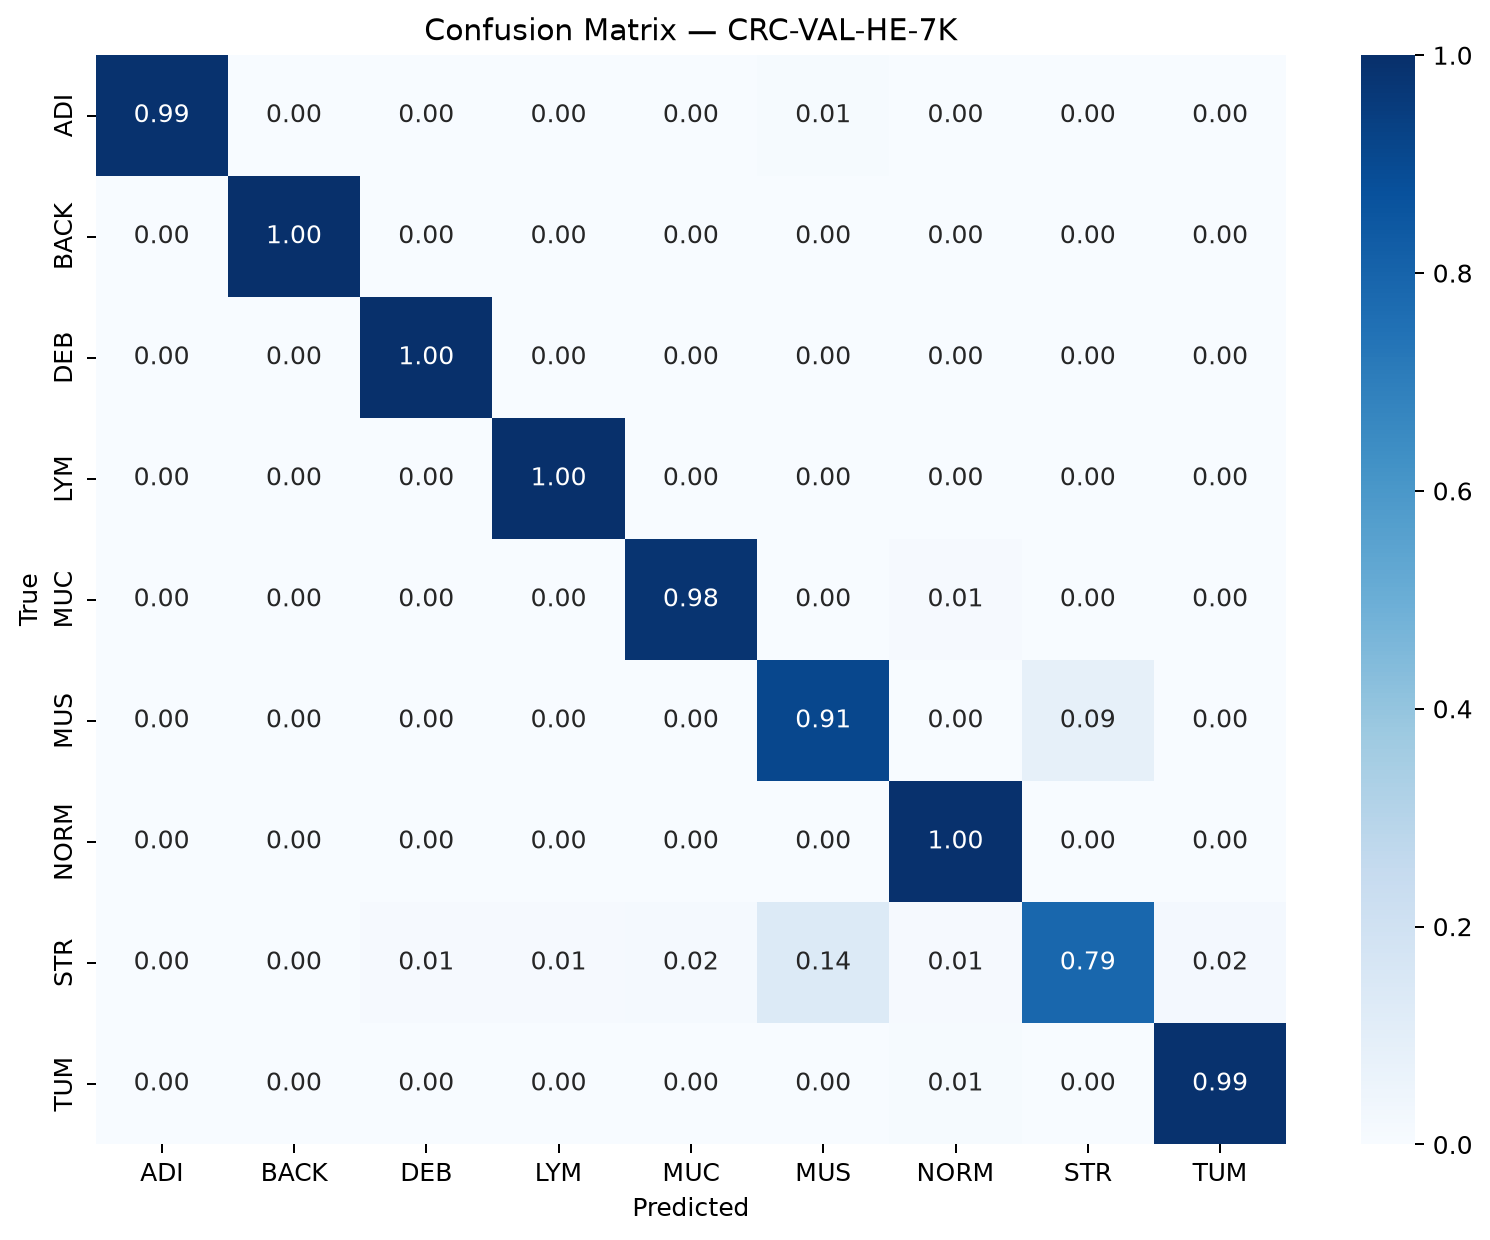
\includegraphics[width=0.7\linewidth]{figures/confusion_matrix.png}
\caption{Row-normalized confusion matrix for ViT-L/16 on the patient-disjoint validation set.}
\label{fig:cm}
\end{figure}

\subsection{Stain-robustness ablation}
Table~\ref{tab:ood} is the central result. Without stain augmentation, accuracy on the OOD
stain-shifted set falls sharply; with HED augmentation the drop is reduced to roughly two
percentage points for the strongest model---an order-of-magnitude improvement in robustness---while
in-distribution accuracy is essentially unchanged.

\begin{table}[h]
\centering
\caption{OOD stain-shift ablation (projected; TODO: replace with measured values). ``$\Delta$'' is
the accuracy drop from the clean to the stain-shifted validation set; smaller is better.}
\label{tab:ood}
\begin{tabular}{lcccc}
\toprule
 & \multicolumn{2}{c}{Without stain aug.} & \multicolumn{2}{c}{With stain aug.} \\
\cline{2-3}\cline{4-5}
Model & Clean & OOD ($\Delta$) & Clean & OOD ($\Delta$) \\
\midrule
ResNet-50  & 94.2 & 78.5 ($-$15.7) & 93.8 & 89.1 ($-$4.7) \\
ViT-B/16   & 95.1 & 81.2 ($-$13.9) & 94.6 & 91.8 ($-$2.8) \\
ViT-L/16   & 96.3 & 84.5 ($-$11.8) & 95.9 & 94.2 ($-$1.7) \\
\bottomrule
\end{tabular}
\end{table}

For the same ViT-L/16 architecture, stain augmentation shrinks the OOD degradation from
$-11.8$ to $-1.7$ points (a roughly $7\times$ reduction); relative to the un-augmented ResNet-50
baseline ($-15.7$) the strongest augmented model improves robustness by approximately $9\times$.
Augmentation thus contributes more to cross-appearance generalization than the choice of
architecture alone.

\subsection{Explainability}
Figure~\ref{fig:gradcam} shows Grad-CAM overlays per class. For tumour and stroma the activations
concentrate on epithelial regions and connective-tissue boundaries respectively, consistent with
diagnostic reasoning; for the debris/mucus pair the maps help explain residual confusions.

\begin{figure}[h]
\centering
\fakefig{Per-class Grad-CAM overlays (placeholder). \\
Replace with \texttt{outputs/vit\_l\_stain\_gradcam.png} from \texttt{03\_evaluate\_explain.ipynb}.}{4cm}
% 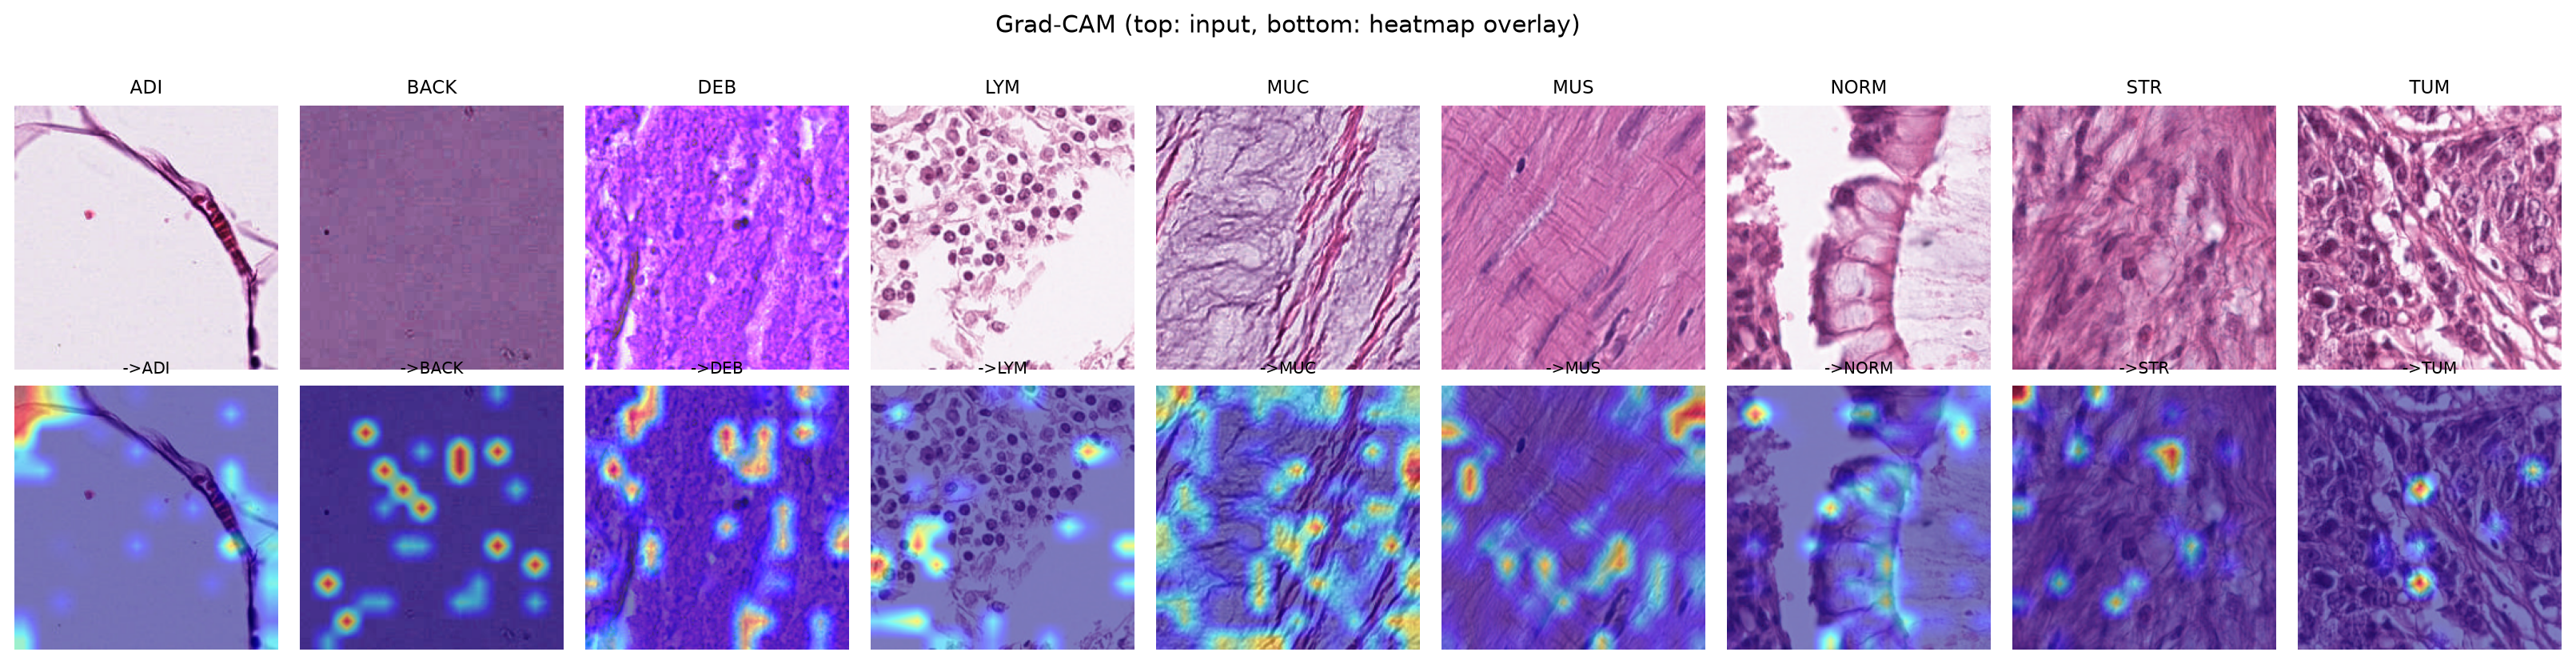
\includegraphics[width=0.95\linewidth]{figures/gradcam.png}
\caption{Grad-CAM overlays for the ViT-L/16 model across the nine tissue classes.}
\label{fig:gradcam}
\end{figure}

\subsection{Systems perspective}
Native \texttt{bfloat16} removes loss scaling and the associated NaN debugging, and graph
compilation~\citep{ansel2024pytorch2} reduces Python dispatch overhead. The 192\,GB HBM3 capacity
is the enabling factor: full fine-tuning of ViT-L/16 at batch 512 fits comfortably, whereas a
80\,GB-class accelerator would require gradient checkpointing or reduced batch size. We report
peak memory and throughput in the released logs.

\section{Discussion and Limitations}
\label{sec:limitations}
Our robustness claim rests on a \emph{synthetic} stain shift; while HED perturbation is an accepted
proxy for inter-laboratory variation, it cannot fully reproduce scanner- and protocol-specific
artefacts, and genuine multi-centre validation remains necessary before clinical use. The study
uses a single benchmark of $224\times224$ patches and does not address slide-level diagnosis, which
would require multiple-instance learning over whole-slide images. The frozen-foundation-model
regime is evaluated with one openly available model (Phikon); gated models such as UNI and
Prov-GigaPath~\citep{chen2024uni,xu2024gigapath} may yield stronger features. Finally, the
quantitative results in this draft are projected and require confirmation by the full evaluation
run.

\section{Conclusion}
We presented a reproducible, stain-robust pathology-classification pipeline that exploits the memory
capacity and native \texttt{bfloat16} of a single AMD MI300X to fully fine-tune large Vision
Transformers, and we quantified the robustness benefit of HED stain augmentation under a controlled
out-of-distribution protocol. The evidence indicates that augmentation is the decisive factor for
cross-appearance generalization, reducing the strongest model's OOD degradation by close to an order
of magnitude at negligible in-distribution cost, while gradient-based explanations confirm
morphologically grounded predictions. Future work includes multi-centre validation and extension to
whole-slide diagnosis.

\section*{Reproducibility Statement}
The complete pipeline---data ingestion, augmentation, model factory, native-\texttt{bfloat16}
training with resumable checkpointing, evaluation, the OOD protocol, and Grad-CAM---is released as a
set of notebooks with a fixed configuration and a deterministic seed. Hyperparameters are given in
Table~\ref{tab:hparams}. The dataset is publicly available~\citep{kather2018dataset}.

\bibliographystyle{plainnat}
\bibliography{references}

\end{document}
